\documentclass[]{book}
\usepackage{lmodern}
\usepackage{amssymb,amsmath}
\usepackage{ifxetex,ifluatex}
\usepackage{fixltx2e} % provides \textsubscript
\ifnum 0\ifxetex 1\fi\ifluatex 1\fi=0 % if pdftex
  \usepackage[T1]{fontenc}
  \usepackage[utf8]{inputenc}
\else % if luatex or xelatex
  \ifxetex
    \usepackage{mathspec}
  \else
    \usepackage{fontspec}
  \fi
  \defaultfontfeatures{Ligatures=TeX,Scale=MatchLowercase}
\fi
% use upquote if available, for straight quotes in verbatim environments
\IfFileExists{upquote.sty}{\usepackage{upquote}}{}
% use microtype if available
\IfFileExists{microtype.sty}{%
\usepackage[]{microtype}
\UseMicrotypeSet[protrusion]{basicmath} % disable protrusion for tt fonts
}{}
\PassOptionsToPackage{hyphens}{url} % url is loaded by hyperref
\usepackage[unicode=true]{hyperref}
\hypersetup{
            pdftitle={Reader-Guigueno Lab Meeting Nov. 4 2020, Project Analyses},
            pdfauthor={Wyatt Toure},
            pdfborder={0 0 0},
            breaklinks=true}
\urlstyle{same}  % don't use monospace font for urls
\usepackage{natbib}
\bibliographystyle{apalike}
\usepackage{color}
\usepackage{fancyvrb}
\newcommand{\VerbBar}{|}
\newcommand{\VERB}{\Verb[commandchars=\\\{\}]}
\DefineVerbatimEnvironment{Highlighting}{Verbatim}{commandchars=\\\{\}}
% Add ',fontsize=\small' for more characters per line
\usepackage{framed}
\definecolor{shadecolor}{RGB}{248,248,248}
\newenvironment{Shaded}{\begin{snugshade}}{\end{snugshade}}
\newcommand{\KeywordTok}[1]{\textcolor[rgb]{0.13,0.29,0.53}{\textbf{#1}}}
\newcommand{\DataTypeTok}[1]{\textcolor[rgb]{0.13,0.29,0.53}{#1}}
\newcommand{\DecValTok}[1]{\textcolor[rgb]{0.00,0.00,0.81}{#1}}
\newcommand{\BaseNTok}[1]{\textcolor[rgb]{0.00,0.00,0.81}{#1}}
\newcommand{\FloatTok}[1]{\textcolor[rgb]{0.00,0.00,0.81}{#1}}
\newcommand{\ConstantTok}[1]{\textcolor[rgb]{0.00,0.00,0.00}{#1}}
\newcommand{\CharTok}[1]{\textcolor[rgb]{0.31,0.60,0.02}{#1}}
\newcommand{\SpecialCharTok}[1]{\textcolor[rgb]{0.00,0.00,0.00}{#1}}
\newcommand{\StringTok}[1]{\textcolor[rgb]{0.31,0.60,0.02}{#1}}
\newcommand{\VerbatimStringTok}[1]{\textcolor[rgb]{0.31,0.60,0.02}{#1}}
\newcommand{\SpecialStringTok}[1]{\textcolor[rgb]{0.31,0.60,0.02}{#1}}
\newcommand{\ImportTok}[1]{#1}
\newcommand{\CommentTok}[1]{\textcolor[rgb]{0.56,0.35,0.01}{\textit{#1}}}
\newcommand{\DocumentationTok}[1]{\textcolor[rgb]{0.56,0.35,0.01}{\textbf{\textit{#1}}}}
\newcommand{\AnnotationTok}[1]{\textcolor[rgb]{0.56,0.35,0.01}{\textbf{\textit{#1}}}}
\newcommand{\CommentVarTok}[1]{\textcolor[rgb]{0.56,0.35,0.01}{\textbf{\textit{#1}}}}
\newcommand{\OtherTok}[1]{\textcolor[rgb]{0.56,0.35,0.01}{#1}}
\newcommand{\FunctionTok}[1]{\textcolor[rgb]{0.00,0.00,0.00}{#1}}
\newcommand{\VariableTok}[1]{\textcolor[rgb]{0.00,0.00,0.00}{#1}}
\newcommand{\ControlFlowTok}[1]{\textcolor[rgb]{0.13,0.29,0.53}{\textbf{#1}}}
\newcommand{\OperatorTok}[1]{\textcolor[rgb]{0.81,0.36,0.00}{\textbf{#1}}}
\newcommand{\BuiltInTok}[1]{#1}
\newcommand{\ExtensionTok}[1]{#1}
\newcommand{\PreprocessorTok}[1]{\textcolor[rgb]{0.56,0.35,0.01}{\textit{#1}}}
\newcommand{\AttributeTok}[1]{\textcolor[rgb]{0.77,0.63,0.00}{#1}}
\newcommand{\RegionMarkerTok}[1]{#1}
\newcommand{\InformationTok}[1]{\textcolor[rgb]{0.56,0.35,0.01}{\textbf{\textit{#1}}}}
\newcommand{\WarningTok}[1]{\textcolor[rgb]{0.56,0.35,0.01}{\textbf{\textit{#1}}}}
\newcommand{\AlertTok}[1]{\textcolor[rgb]{0.94,0.16,0.16}{#1}}
\newcommand{\ErrorTok}[1]{\textcolor[rgb]{0.64,0.00,0.00}{\textbf{#1}}}
\newcommand{\NormalTok}[1]{#1}
\usepackage{longtable,booktabs}
% Fix footnotes in tables (requires footnote package)
\IfFileExists{footnote.sty}{\usepackage{footnote}\makesavenoteenv{long table}}{}
\usepackage{graphicx,grffile}
\makeatletter
\def\maxwidth{\ifdim\Gin@nat@width>\linewidth\linewidth\else\Gin@nat@width\fi}
\def\maxheight{\ifdim\Gin@nat@height>\textheight\textheight\else\Gin@nat@height\fi}
\makeatother
% Scale images if necessary, so that they will not overflow the page
% margins by default, and it is still possible to overwrite the defaults
% using explicit options in \includegraphics[width, height, ...]{}
\setkeys{Gin}{width=\maxwidth,height=\maxheight,keepaspectratio}
\IfFileExists{parskip.sty}{%
\usepackage{parskip}
}{% else
\setlength{\parindent}{0pt}
\setlength{\parskip}{6pt plus 2pt minus 1pt}
}
\setlength{\emergencystretch}{3em}  % prevent overfull lines
\providecommand{\tightlist}{%
  \setlength{\itemsep}{0pt}\setlength{\parskip}{0pt}}
\setcounter{secnumdepth}{5}
% Redefines (sub)paragraphs to behave more like sections
\ifx\paragraph\undefined\else
\let\oldparagraph\paragraph
\renewcommand{\paragraph}[1]{\oldparagraph{#1}\mbox{}}
\fi
\ifx\subparagraph\undefined\else
\let\oldsubparagraph\subparagraph
\renewcommand{\subparagraph}[1]{\oldsubparagraph{#1}\mbox{}}
\fi

% set default figure placement to htbp
\makeatletter
\def\fps@figure{htbp}
\makeatother

\usepackage{booktabs}

\title{Reader-Guigueno Lab Meeting Nov. 4 2020, Project Analyses}
\author{Wyatt Toure}
\date{2020-11-02}

\begin{document}
\maketitle

{
\setcounter{tocdepth}{1}
\tableofcontents
}
\chapter{Background}\label{background}

Based on previous literature we have good reason to believe two things
about guppy exploratory behaviour, defined as the propensity to engage
with novelty:

\begin{itemize}
\tightlist
\item
  that there is a relatively \textbf{strong environmenetal component to
  exploratory behaviour} (Burns \emph{et. al.} 2016)
\item
  that \textbf{exploratory tendencies across contexts are correlated}
  (De Serrano \emph{et al.} 2016)
\end{itemize}

My experiments try to examine whether there is a role for experience in
the environment in shaping exploratory behaviour and to look at the
implications of a potential behavioural corrrelation across novelty
contexts. If exploratory tendencies are correlated across contexts
because of shared mechanisms producing both behaviours then shifting
exploration in one context should also shift exploratory tendencies in
another context even without directly training for exploration in that
context.

To tackle these quesitons I have tried to shift novel object exploration
and spatial exploration through reinforcement training.

I took a stepwise approach to this. Before I asked whether I could shift
novel object preferences I wanted to confirm that:

\begin{itemize}
\tightlist
\item
  { Guppies recognize and respond to novel objects }
\item
  Guppies can have their preference for objects shifted
\end{itemize}

After confirming those I then felt comfortable to go on and see if I
could shift \emph{novel} object preferences.

\chapter{Project 1 --- General Methods}\label{methods}

\textbf{Question}: Can I shift the preference for a particular object by
reinforcing an object with a food reward.

I had one set of guppies trained to the blue object (blue-trained
guppies) and another set trained to the green object (green-trained
guppies).

I performed the following trials:

\begin{itemize}
\tightlist
\item
   1 baseline object preference test (Guppy in tank with 1 green and 1
  blue object, unrewarded)
\item
   20 training trials (Guppy in tank with 1 green and 1 blue object,
  rewarded for visiting one or the other based on treatment)
\item
   1 final object preference test (Guppy in tank with 1 green and 1 blue
  object, unrewarded)
\end{itemize}

\chapter{Model 1 - Preference for the green object at
baseline}\label{model-1---preference-for-the-green-object-at-baseline}

\begin{Shaded}
\begin{Highlighting}[]
\NormalTok{baseline.data.model =}\StringTok{ }
\StringTok{  }\KeywordTok{lm}\NormalTok{(green.object.preference }\OperatorTok{~}\StringTok{ }\DecValTok{1}\NormalTok{,}
     \DataTypeTok{data =}\NormalTok{ baseline.data)}
\end{Highlighting}
\end{Shaded}

At baseline, there was no significant difference in green object
preference betweeen the treatments (p = 0.727).

\chapter{Model 2 - Preference for the rewarding object during
training}\label{model-2---preference-for-the-rewarding-object-during-training}

To see whether fish were responsive during training our second model
asks whether the preference for the rewarding object changes throughout
training between the treatments.

\begin{Shaded}
\begin{Highlighting}[]
\NormalTok{training.data.model =}\StringTok{ }
\StringTok{  }\KeywordTok{lmer}\NormalTok{(rewarding.object.preference }\OperatorTok{~}\StringTok{ }\NormalTok{rewarding.object.colour }\OperatorTok{*}\StringTok{ }\NormalTok{trial }\OperatorTok{+}\StringTok{ }\NormalTok{(}\DecValTok{1} \OperatorTok{|}\StringTok{ }\NormalTok{id), }
       \DataTypeTok{data =}\NormalTok{ training.data)}
\end{Highlighting}
\end{Shaded}

\begin{verbatim}
## # A tibble: 3 x 6
##   term                               estimate std.error statistic    df p.value
##   <chr>                                 <dbl>     <dbl>     <dbl> <dbl> <chr>  
## 1 rewarding.object.colourgreen         56.0       27.3      2.05   47.2 0.046  
## 2 trial                                 7.70       1.08     7.10  438.  < .001 
## 3 rewarding.object.colourgreen:trial   -0.549      1.49    -0.368 435.  0.713
\end{verbatim}

Throughout training, over the 20 trials, guppies increased their
relative preference for the rewarded object by 7.7 seconds each trial
(Figure \ref{fig:novel-pref-plot}, p \textless{} .001).

\begin{figure}
\centering
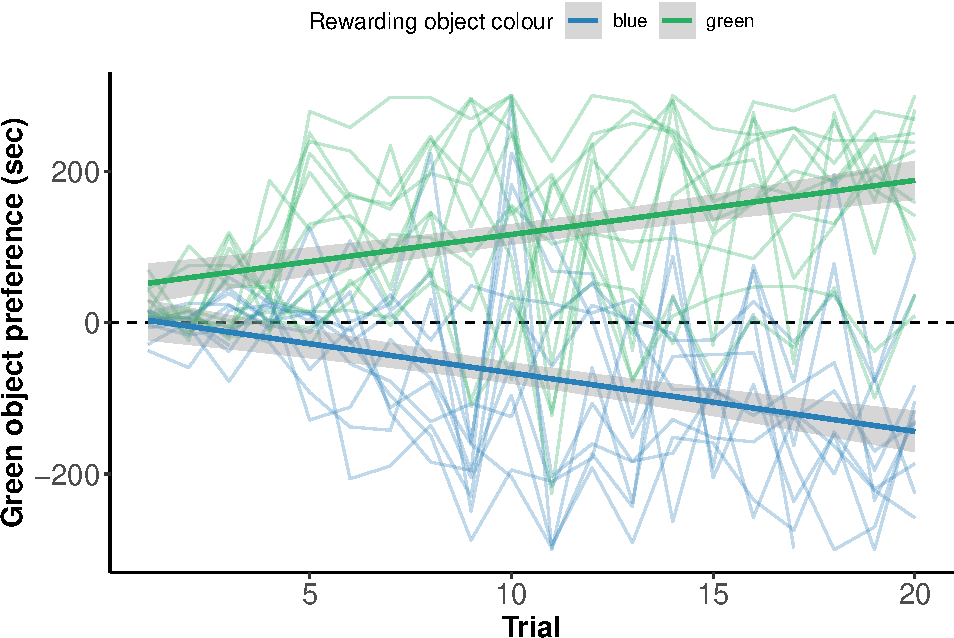
\includegraphics{nov-4-2020-lab-meeting-on-analyses_files/figure-latex/novel-pref-plot-1.pdf}
\caption{\label{fig:novel-pref-plot}Preference for the green object in both
treatments. Negative values represent more time spent with the blue
object, positive values indicate more time spent with the green object.
Faded lines connect individuals across trials and solid lines represents
a linear fit with 95\% CI (grey shading).}
\end{figure}

\chapter{Model 3 - Preference for the rewarded object during testing
depending on
treatment}\label{model-3---preference-for-the-rewarded-object-during-testing-depending-on-treatment}

For the main effects of \textbf{training} and \textbf{rewarding object
colour} on object preference I fit a \textbf{linear mixed effects model}
with \textbf{fixed effects of trial} and \textbf{rewarding object
colour} and a random effect of \textbf{individual id}. My third model
asks whether the preference for the rewarding object changed between
baseline and final test and looks for an interaction with rewarded
object colour.

\begin{Shaded}
\begin{Highlighting}[]
\NormalTok{test.data.model =}\StringTok{ }
\StringTok{  }\KeywordTok{lmer}\NormalTok{(rewarding.object.preference }\OperatorTok{~}\StringTok{ }\NormalTok{rewarding.object.colour }\OperatorTok{*}\StringTok{ }\NormalTok{trial }\OperatorTok{+}\StringTok{ }\NormalTok{(}\DecValTok{1} \OperatorTok{|}\StringTok{ }\NormalTok{id),}
       \DataTypeTok{data =}\NormalTok{ test.data)}
\end{Highlighting}
\end{Shaded}

\begin{verbatim}
## # A tibble: 3 x 6
##   term                                estimate std.error statistic    df p.value
##   <chr>                                  <dbl>     <dbl>     <dbl> <dbl> <chr>  
## 1 rewarding.object.colourgreen            1.64      16.3     0.101  39.9 0.92   
## 2 trial21                                17.7       16.6     1.06   20.0 0.3    
## 3 rewarding.object.colourgreen:trial~    65.4       22.5     2.90   20.0 0.009
\end{verbatim}

I found a significant interaction effect between trial and rewarding
object colour (p = 0.009). Guppies that had green rewarded had a
rewarded object preference that was 65.4 seconds stronger than the
rewarded object preference of guppies trained to blue (Figure
\ref{fig:test-data-pref-plot}).

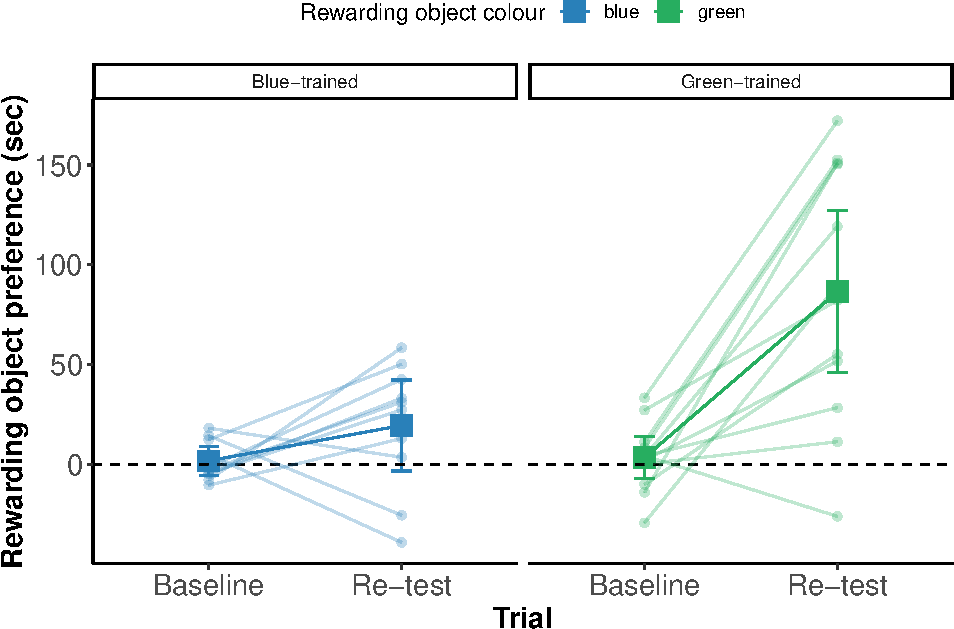
\includegraphics{nov-4-2020-lab-meeting-on-analyses_files/figure-latex/test-data-pref-plot-1.pdf}

Post-hoc pairwise comparisons investigating the differences between
treatments based on whether guppies are untrained or trained reveals
that initially there was no difference in the strength of preference for
the rewarding object between the treatments (blue-trained guppies had a
blue object preference of 1.8 seconds and green-trained guppies had a
green object preference of 3.5 seconds, p = 1).

Comparing the shift in rewarding object preference between initial and
final preference tests in blue-trained and green-trained guppies reveals
that the shift in rewarding object preference is significant for
green-trained guppies but not for blue-trained guppies. Green trained
guppies increased their preference for the green object by 83 seconds
(going from a green object preference of 3.5 seconds initially to 86.5
seconds at final test, p \textless{} .001) whereas blue-trained guppies
non-significantly increased their preference for the blue object by 17.7
seconds (going from a blue object preference 1.8 seconds initially to
19.5 seconds at final test, p = 0.714). For a full description of
post-hoc comparisons see table \ref{tab:contrasts-table}.

\begin{enumerate}
\def\labelenumi{\arabic{enumi}.}
\tightlist
\item
  Green-trained guppies increased their preference for the green object.
\item
  Blue-trained guppies non-significantly increased their preference for
  the blue object. 
\end{enumerate}

\begin{table}

\caption{\label{tab:contrasts-table}Table of post-hoc tests with Tukey adjustment for multiple comparisons. The numbers represent the initial test trial (0) and the final test trial (21). The colour corressponds to the identity of the rewarding object (blue for blue-trained guppies, green for green-trained guppies). Values are all rounded to 3 decimal places. Significant p-values are bolded.}
\centering
\begin{tabular}[t]{l|r|r|r|r|l}
\hline
contrast & estimate & df & lower.CL & upper.CL & p.value\\
\hline
0 blue - 21 blue & -17.697 & 20.000 & -64.236 & 28.842 & 0.714\\
\hline
0 blue - 0 green & -1.645 & 39.908 & -45.381 & 42.092 & 1\\
\hline
0 blue - 21 green & -84.693 & 39.908 & -128.429 & -40.956 & **< .001**\\
\hline
21 blue - 0 green & 16.052 & 39.908 & -27.684 & 59.789 & 0.759\\
\hline
21 blue - 21 green & -66.996 & 39.908 & -110.732 & -23.259 & 0.001\\
\hline
0 green - 21 green & -83.048 & 20.000 & -125.532 & -40.564 & **< .001**\\
\hline
\end{tabular}
\end{table}

\chapter{Model 4 - Preference for the rewarded object during training
based on
feeding}\label{model-4---preference-for-the-rewarded-object-during-training-based-on-feeding}

My fourth model asks whether the time spent near the rewarding object
during a training session is influenced by whether a fish ate or not.

\begin{Shaded}
\begin{Highlighting}[]
\NormalTok{training.data.model.rewarding.object =}\StringTok{ }
\StringTok{  }\KeywordTok{lmer}\NormalTok{(rewarding.object.preference }\OperatorTok{~}\StringTok{ }\NormalTok{ate }\OperatorTok{+}\StringTok{ }\NormalTok{(}\DecValTok{1} \OperatorTok{|}\StringTok{ }\NormalTok{id) }\OperatorTok{+}\StringTok{ }\NormalTok{(}\DecValTok{1} \OperatorTok{|}\StringTok{ }\NormalTok{trial),}
       \DataTypeTok{data =}\NormalTok{ training.data)}
\end{Highlighting}
\end{Shaded}

\begin{verbatim}
## # A tibble: 1 x 6
##   term   estimate std.error statistic    df p.value
##   <chr>     <dbl>     <dbl>     <dbl> <dbl> <chr>  
## 1 ateyes     91.2      11.0      8.33  224. < .001
\end{verbatim}

Throughout all of training, fish that ate during a session spent on
average 91.2 more seconds near the rewarded object compared to fish that
did not eat (Figure, \ref{fig:training-data-ate-plot}, p \textless{}
.001). Fish that spent more trials eating may therefore have received
more reinforcement for the object-food association.

\begin{figure}
\centering
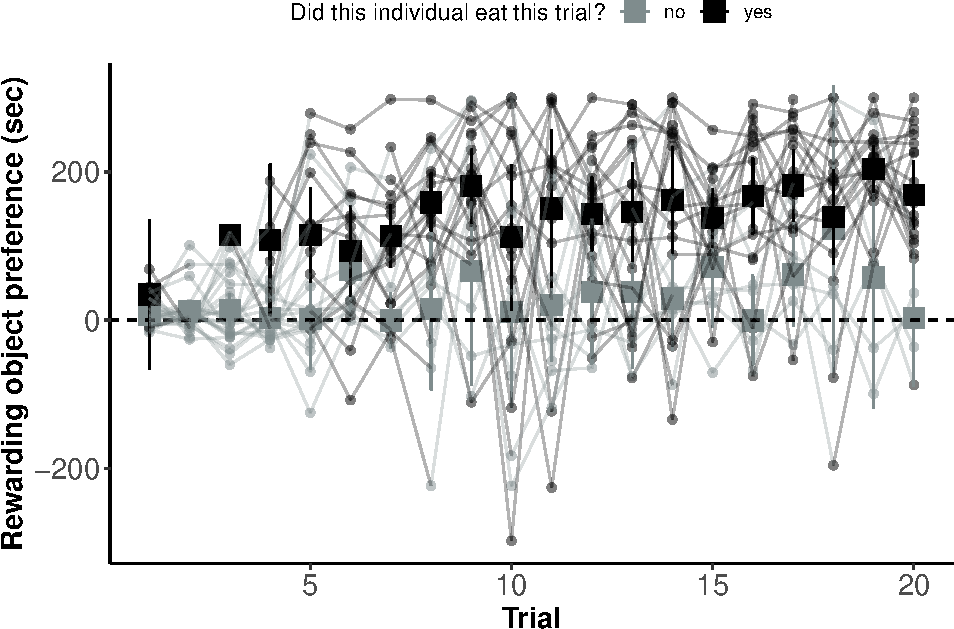
\includegraphics{nov-4-2020-lab-meeting-on-analyses_files/figure-latex/training-data-ate-plot-1.pdf}
\caption{\label{fig:training-data-ate-plot}Preference for the rewarding
object during training based on whether an individual ate during a trial
or not. Dashed line represents the no preference value. Data are means
+/- 95\% CI.}
\end{figure}

A discrepancy in reinforcement between treatments may influence
performance on a final preference test. To see whether there was a
difference in feeding between treatments I counted the number of trials
in which an individual fish ate throughout all of training and compared
the feeding counts between treatments. To do this I fit a generalized
linear model with a Poisson distribution.

\chapter{Model 5 - Is there a difference in feeding attempts between
treatments?}\label{model-5---is-there-a-difference-in-feeding-attempts-between-treatments}

\begin{Shaded}
\begin{Highlighting}[]
\NormalTok{feeding.data.model =}\StringTok{ }
\StringTok{  }\KeywordTok{glm}\NormalTok{(feeding.count }\OperatorTok{~}\StringTok{ }\NormalTok{rewarding.object.colour, }\DataTypeTok{family =} \StringTok{"poisson"}\NormalTok{, }
      \DataTypeTok{data =}\NormalTok{ my.feeding.data)}
\end{Highlighting}
\end{Shaded}

The response variable `feeding count' is a sum of the number of trials
in which a guppy ate.

\begin{verbatim}
## # A tibble: 1 x 5
##   term                         estimate std.error statistic p.value
##   <chr>                           <dbl>     <dbl>     <dbl> <chr>  
## 1 rewarding.object.colourgreen   0.0710     0.126     0.561 0.575
\end{verbatim}

I found no significant difference in the amount of feeding done by
individuals trained to green versus individuals trained to blue (Figure
\ref{fig:feeding-count-plot}, p = 0.575) which suggests that the
observed group-level differences in final test performance between
blue-trained guppies versus green-trained guppies cannot be explained by
differences in performance during training.

\begin{figure}
\centering
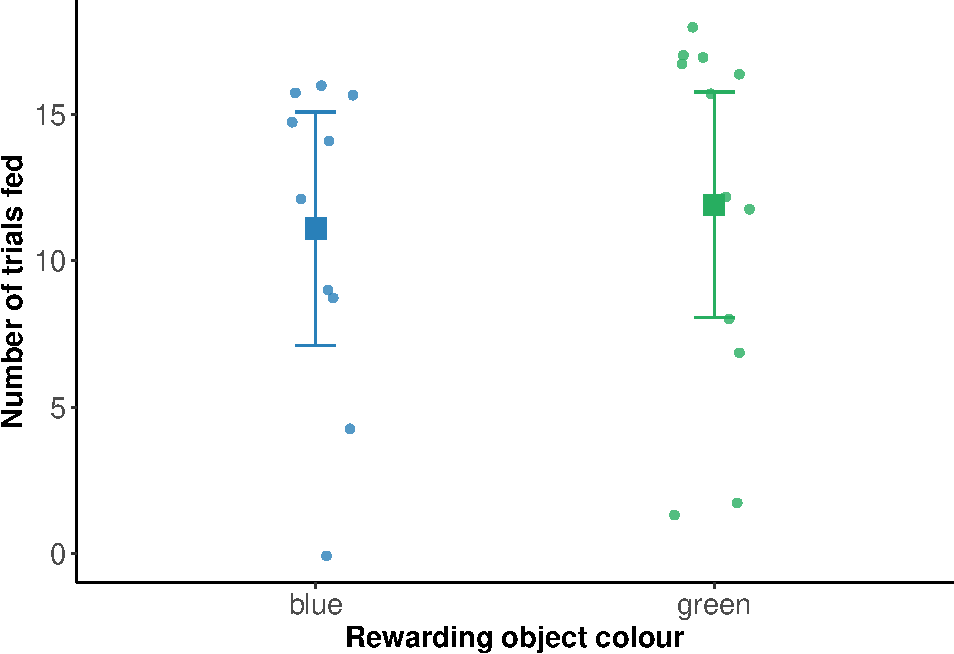
\includegraphics{nov-4-2020-lab-meeting-on-analyses_files/figure-latex/feeding-count-plot-1.pdf}
\caption{\label{fig:feeding-count-plot}Average number of trials in which a
fish fed during training. Data are means +/- 95\% confidence intervals}
\end{figure}

\chapter{Model 6 - What if I control for feeding
count?}\label{model-6---what-if-i-control-for-feeding-count}

\begin{Shaded}
\begin{Highlighting}[]
\NormalTok{test.data.feeding.controlled.model =}\StringTok{ }
\StringTok{  }\KeywordTok{lm}\NormalTok{(rewarding.object.preference }\OperatorTok{~}\StringTok{ }\NormalTok{trial }\OperatorTok{*}\StringTok{ }\NormalTok{rewarding.object.colour }\OperatorTok{+}\StringTok{ }\NormalTok{feeding.count, }
     \DataTypeTok{data =}\NormalTok{ test.feeding.data)}
\end{Highlighting}
\end{Shaded}

\begin{verbatim}
## # A tibble: 4 x 5
##   term                                 estimate std.error statistic p.value
##   <chr>                                   <dbl>     <dbl>     <dbl> <chr>  
## 1 trial21                                17.7       16.9     1.05   0.301  
## 2 rewarding.object.colourgreen            0.538     16.2     0.0332 0.974  
## 3 feeding.count                           1.36       1.02    1.33   0.192  
## 4 trial21:rewarding.object.colourgreen   65.4       22.9     2.86   0.007
\end{verbatim}

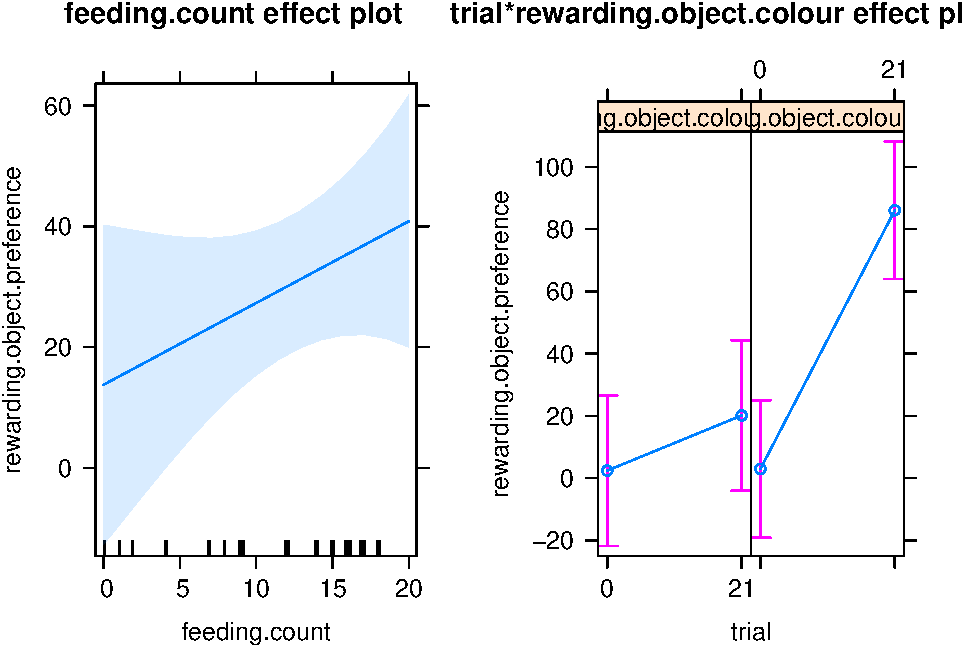
\includegraphics{nov-4-2020-lab-meeting-on-analyses_files/figure-latex/unnamed-chunk-13-1.pdf}

Nothing changes if I control for feeding count.

\chapter{Model 7 - Does feeding count predict
anything?}\label{model-7---does-feeding-count-predict-anything}

\begin{Shaded}
\begin{Highlighting}[]
\NormalTok{test.data.feeding.controlled.model1 =}\StringTok{ }
\StringTok{  }\KeywordTok{lm}\NormalTok{(rewarding.object.preference }\OperatorTok{~}\StringTok{ }\NormalTok{feeding.count,}
     \DataTypeTok{data =}\NormalTok{ retest.feeding.data)}
\end{Highlighting}
\end{Shaded}

\begin{verbatim}
## # A tibble: 1 x 5
##   term          estimate std.error statistic p.value
##   <chr>            <dbl>     <dbl>     <dbl> <chr>  
## 1 feeding.count     2.62      2.32      1.13 0.272
\end{verbatim}

Testing for an effect of feeding count on rewarding object preference
finds that there is no significant effect but the effect is in the
expected direction.

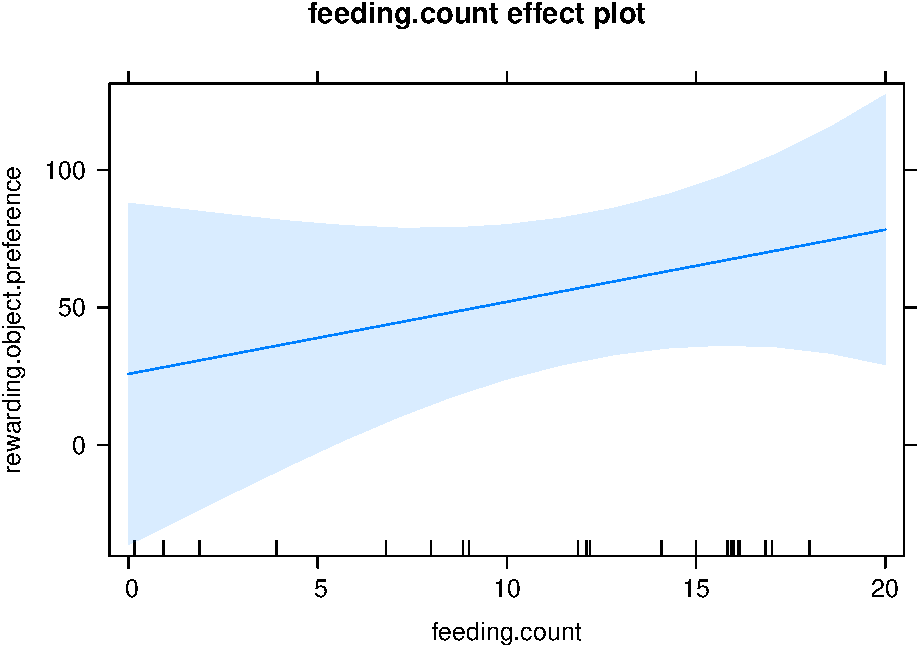
\includegraphics{nov-4-2020-lab-meeting-on-analyses_files/figure-latex/unnamed-chunk-16-1.pdf}

However,there is an effect of feeding on the time spent near
\textbf{both} objects at re-test.

\begin{Shaded}
\begin{Highlighting}[]
\NormalTok{test.data.feeding.controlled.model2 =}\StringTok{ }
\StringTok{  }\KeywordTok{lm}\NormalTok{(time.with.both.objects }\OperatorTok{~}\StringTok{ }\NormalTok{feeding.count,}
     \DataTypeTok{data =}\NormalTok{ retest.feeding.data)}
\end{Highlighting}
\end{Shaded}

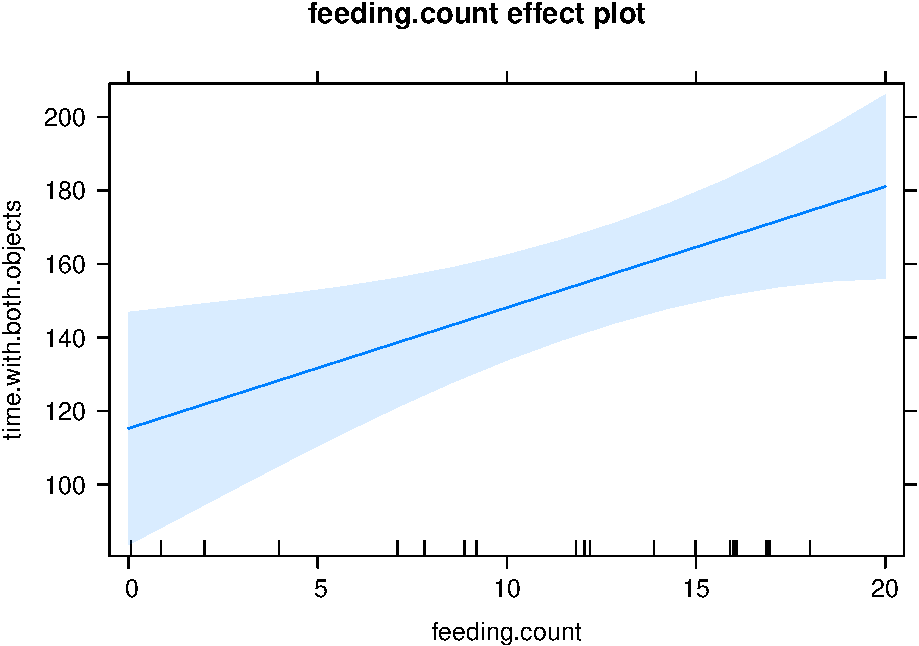
\includegraphics{nov-4-2020-lab-meeting-on-analyses_files/figure-latex/unnamed-chunk-18-1.pdf}

During the final test, a fish that had 0 feedings spent 115.299 seconds
near both objects whereas fish that fed in 20 trials spent 181.009
seconds near both objects, a 1.6-fold increase.

\chapter{An interesting trend from a very early
pilot}\label{an-interesting-trend-from-a-very-early-pilot}

\begin{figure}
\centering
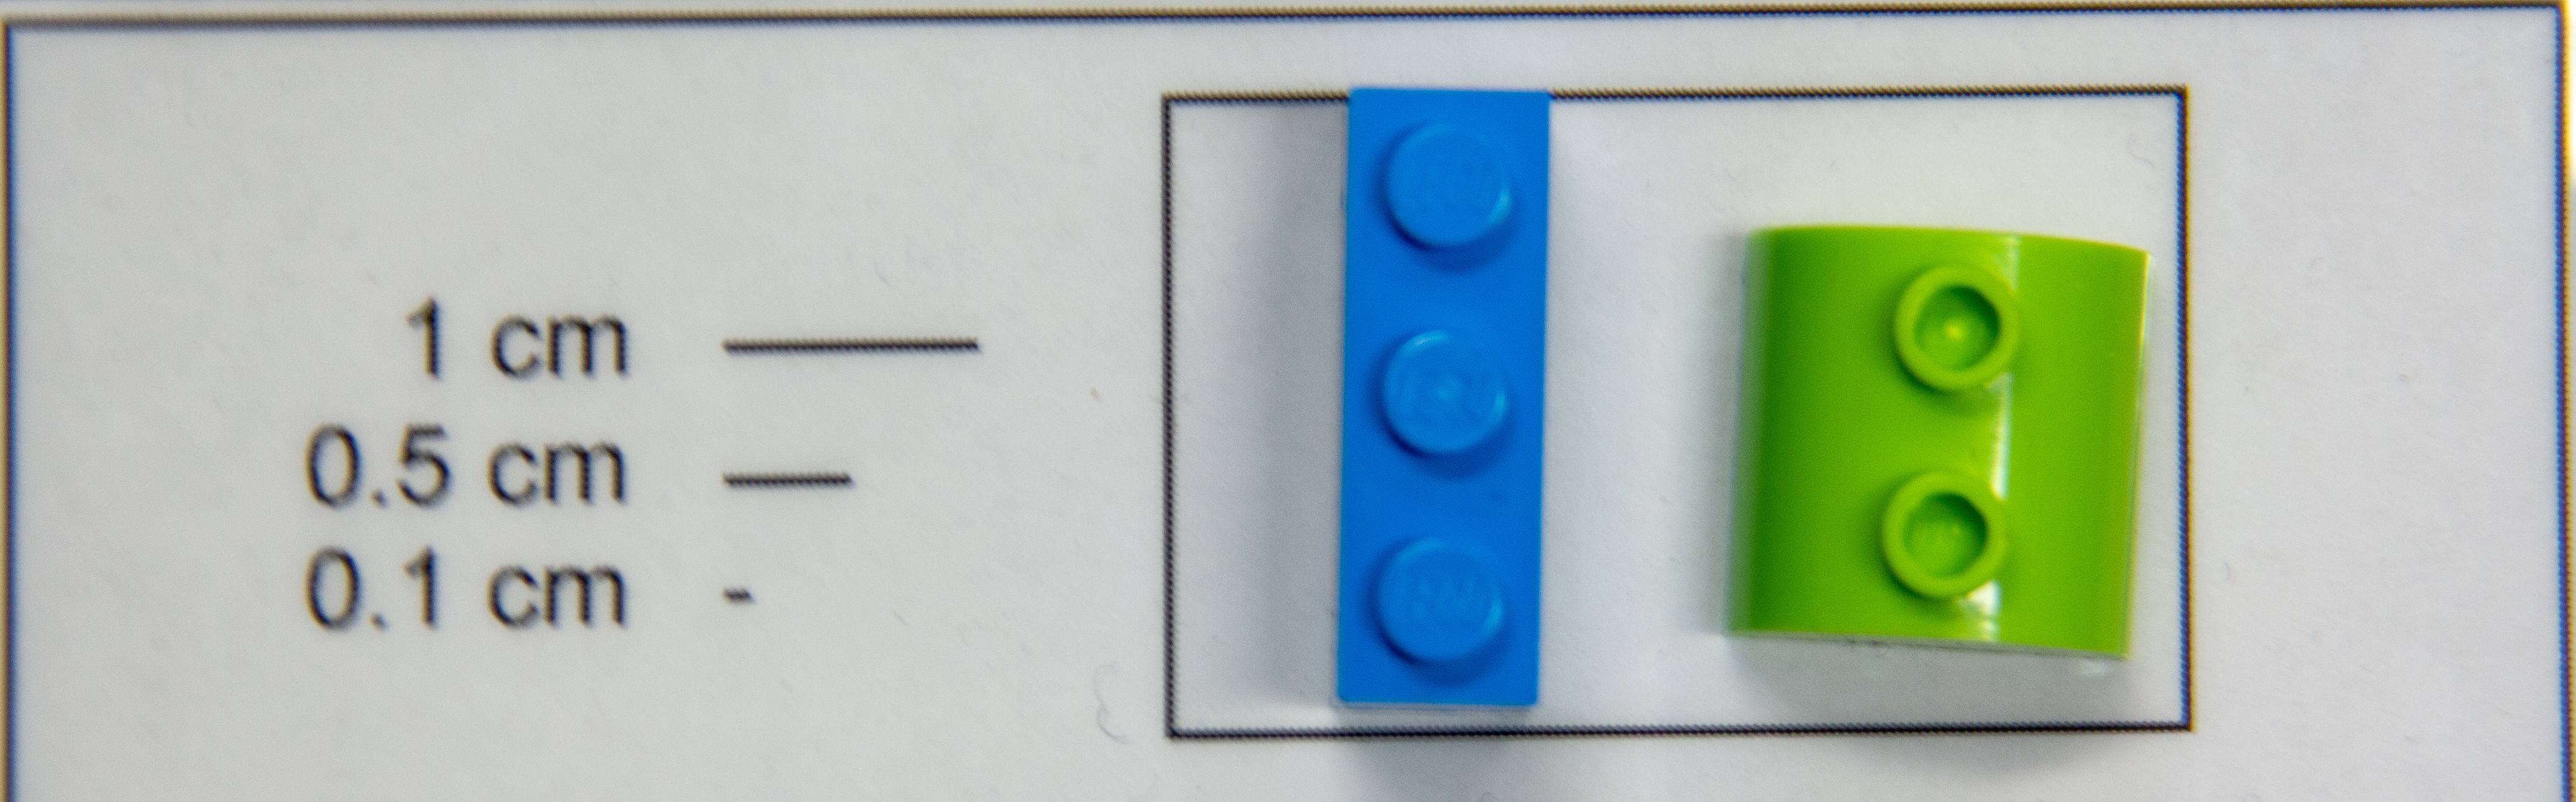
\includegraphics{images/objects.jpg}
\caption{Objects from a very early experiment}
\end{figure}

\begin{Shaded}
\begin{Highlighting}[]
\NormalTok{pilot.model =}\StringTok{ }
\StringTok{  }\KeywordTok{lmer}\NormalTok{(time.with.trained.object }\OperatorTok{~}\StringTok{ }\NormalTok{trial }\OperatorTok{*}\StringTok{ }\NormalTok{object.colour }\OperatorTok{+}\StringTok{ }\NormalTok{(}\DecValTok{1} \OperatorTok{|}\StringTok{ }\NormalTok{id), }
       \DataTypeTok{data =}\NormalTok{ pilot.data)}
\end{Highlighting}
\end{Shaded}

\begin{verbatim}
## # A tibble: 7 x 6
##   term                        estimate std.error statistic    df p.value
##   <chr>                          <dbl>     <dbl>     <dbl> <dbl> <chr>  
## 1 trial11:object.colourgreen    24.5        12.0    2.04    26.6 0.052  
## 2 trial11:object.colourgrey      0.300      16.1    0.0186  26.6 0.985  
## 3 trial11:object.colourorange   12.7        16.1    0.787   26.6 0.438  
## 4 trial11:object.colourpurple    2.50       18.6    0.134   26.6 0.894  
## 5 trial11:object.colourred      25.9        16.1    1.60    26.6 0.121  
## 6 trial11:object.colourwhite    11.6        17.7    0.659   30.4 0.515  
## 7 trial11:object.colouryellow   -1.63       13.2   -0.124   26.6 0.902
\end{verbatim}

\begin{verbatim}
##  model: time.with.trained.object ~ trial * object.colour
## 
##  trial*object.colour effect
##      object.colour
## trial     blue    green     grey   orange  purple      red    white   yellow
##    0  56.22172 47.98031 39.63883 53.18540 46.2453 43.50927 54.78697 64.86343
##    11 46.11182 62.37222 29.82920 55.78797 38.6378 59.25800 56.31596 53.11867
\end{verbatim}

\chapter{Project 2 --- General methods}\label{project-2-general-methods}

In this experiment I performed the following trials:

\begin{itemize}
\tightlist
\item
  2 baseline open field tests (Guppy in empty 5 gallon tank)
\item
  3 baseline object exploration tests (Guppy in 5 gallon tank with 1
  familiar object and 1 novel object)
\item
  2 baseline maze exploration tests (Guppy in 20 gallon tank with 16
  compartments)
\item
  20 training trials training guppies to novel or familiar objects
  (Guppy in 5 gallon tank with 1 familiar object and 1 novel object)
\item
  3 object exploration re-tests (Guppy in 5 gallon tank with 1 familiar
  object and 1 novel object)
\item
  2 maze exploration re-tests (Guppy in 20 gallon tank with 16
  compartments)
\item
  1 mate preference test (Female guppy in 5 gallon tank with 1 familiar
  male and 1 novel novel)
\end{itemize}

This analysis so far focuses on the object exploraiton tests and
training with the incorporation of spatial exploration and mate
preference pending.

\begin{figure}
\centering
\includegraphics{images/sample-fish-trial.gif}
\caption{Sample footage of an expeimental trial}
\end{figure}

\chapter{Model 1 - Preference for the novel object at
baseline}\label{model-1---preference-for-the-novel-object-at-baseline}

\begin{Shaded}
\begin{Highlighting}[]
\NormalTok{baseline.data.model =}\StringTok{ }
\StringTok{  }\KeywordTok{lmer}\NormalTok{(novel.object.preference }\OperatorTok{~}\StringTok{ }\DecValTok{1} \OperatorTok{+}\StringTok{ }\NormalTok{(}\DecValTok{1}\OperatorTok{|}\NormalTok{id) }\OperatorTok{+}\StringTok{ }\NormalTok{(}\DecValTok{1}\OperatorTok{|}\NormalTok{trial), }
       \DataTypeTok{data =}\NormalTok{ baseline.data)}
\end{Highlighting}
\end{Shaded}

\begin{verbatim}
## boundary (singular) fit: see ?isSingular
\end{verbatim}

There is no significant preference for the novel object over the
familiar object at baseline (p = 0.491). There is a singular fit and
closer inspection reveals that the individual ID random effect is not
capturing any variance (id standard deviation = 0 whereas the trial
standard deviation = 29.531).

\chapter{Baseline repeatabilities}\label{baseline-repeatabilities}

\begin{Shaded}
\begin{Highlighting}[]
\CommentTok{# Repeatability of time in center of the tank during open field baseline }

\NormalTok{time.in.center.repeatability.open.field =}\StringTok{ }
\StringTok{  }\KeywordTok{rpt}\NormalTok{(time.in.center }\OperatorTok{~}\StringTok{ }\NormalTok{(}\DecValTok{1} \OperatorTok{|}\StringTok{ }\NormalTok{id), }\DataTypeTok{grname =} \StringTok{"id"}\NormalTok{, }\DataTypeTok{datatype =} \StringTok{"Gaussian"}\NormalTok{,}
      \DataTypeTok{data =}\NormalTok{ open.field.data, }\DataTypeTok{nboot =} \DecValTok{50}\NormalTok{ , }\DataTypeTok{npermut =} \DecValTok{0}\NormalTok{) }
\end{Highlighting}
\end{Shaded}

During the first two trials, the open field baselines, time in center is
highly repeatable (R = 0.651, p \textless{} 0.001).

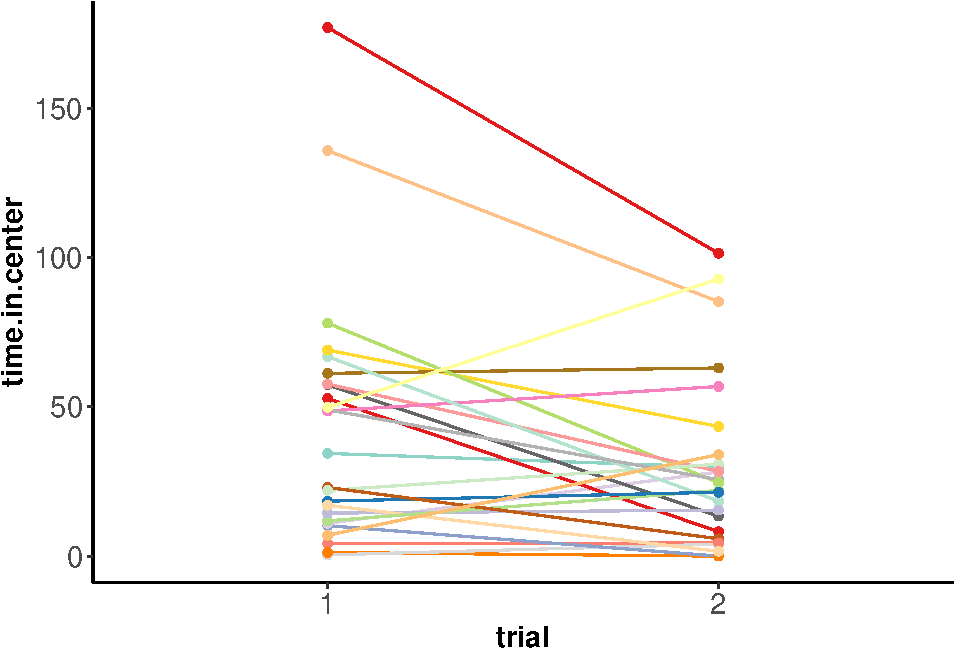
\includegraphics{nov-4-2020-lab-meeting-on-analyses_files/figure-latex/unnamed-chunk-26-1.pdf}

\begin{Shaded}
\begin{Highlighting}[]
\CommentTok{# Repeatability of activity during open field baseline }
\NormalTok{activity.repeatability.open.field =}\StringTok{ }
\StringTok{  }\KeywordTok{rpt}\NormalTok{(distance.moved }\OperatorTok{~}\StringTok{ }\NormalTok{(}\DecValTok{1} \OperatorTok{|}\StringTok{ }\NormalTok{id), }\DataTypeTok{grname =} \StringTok{"id"}\NormalTok{, }\DataTypeTok{datatype =} \StringTok{"Gaussian"}\NormalTok{, }
      \DataTypeTok{data =}\NormalTok{ open.field.data, }\DataTypeTok{nboot =} \DecValTok{50}\NormalTok{ , }\DataTypeTok{npermut =} \DecValTok{0}\NormalTok{) }
\end{Highlighting}
\end{Shaded}

During the open field baselines general activity is not repeatable, (R =
0.253, p = 0.118)

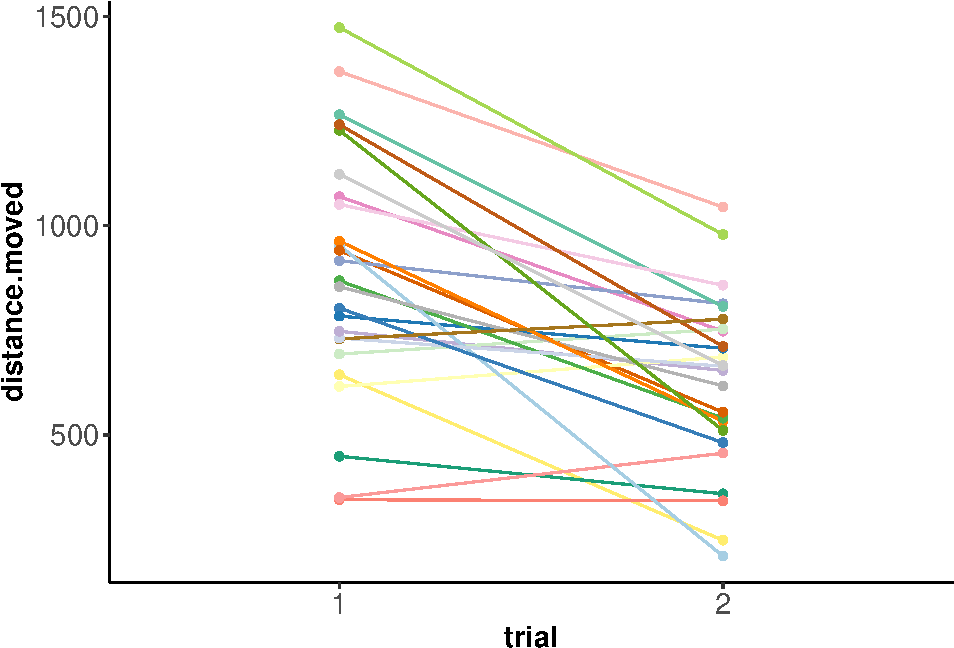
\includegraphics{nov-4-2020-lab-meeting-on-analyses_files/figure-latex/unnamed-chunk-29-1.pdf}

\begin{Shaded}
\begin{Highlighting}[]
\CommentTok{# Repeatability of activity during novel object exploration baseline }
\NormalTok{activity.repeatability =}\StringTok{ }
\StringTok{  }\KeywordTok{rpt}\NormalTok{(distance.moved }\OperatorTok{~}\StringTok{ }\NormalTok{(}\DecValTok{1} \OperatorTok{|}\StringTok{ }\NormalTok{id), }\DataTypeTok{grname =} \StringTok{"id"}\NormalTok{, }\DataTypeTok{datatype =} \StringTok{"Gaussian"}\NormalTok{, }
      \DataTypeTok{data =}\NormalTok{ baseline.data, }\DataTypeTok{nboot =} \DecValTok{50}\NormalTok{ , }\DataTypeTok{npermut =} \DecValTok{0}\NormalTok{)}
\end{Highlighting}
\end{Shaded}

General activity was repeatable during the novel object baseline assays
R = 0.464 (95\% CI = 0.203, 0.631, p = 0).
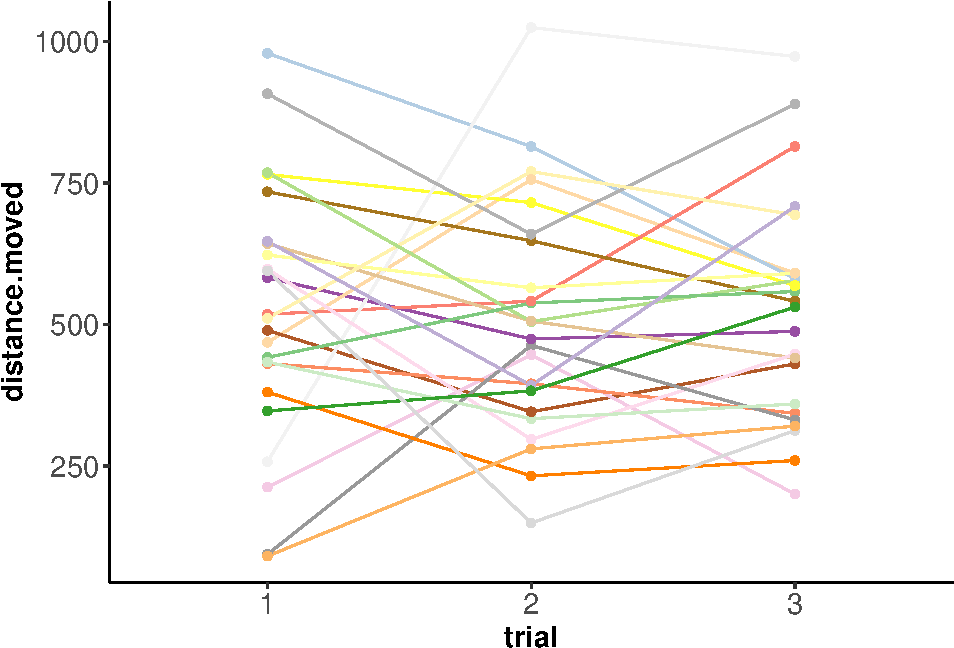
\includegraphics{nov-4-2020-lab-meeting-on-analyses_files/figure-latex/unnamed-chunk-33-1.pdf}

\begin{Shaded}
\begin{Highlighting}[]
\CommentTok{# Repeatability of time spent near novel object at baseline }
\NormalTok{novel.object.pref.rpt =}\StringTok{ }
\StringTok{  }\KeywordTok{rpt}\NormalTok{(time.with.novel.object }\OperatorTok{~}\StringTok{ }\NormalTok{(}\DecValTok{1} \OperatorTok{|}\StringTok{ }\NormalTok{id), }\DataTypeTok{grname =} \StringTok{"id"}\NormalTok{, }\DataTypeTok{datatype =} \StringTok{"Gaussian"}\NormalTok{, }
      \DataTypeTok{data =}\NormalTok{ baseline.data, }\DataTypeTok{nboot =} \DecValTok{50}\NormalTok{ , }\DataTypeTok{npermut =} \DecValTok{0}\NormalTok{) }
\end{Highlighting}
\end{Shaded}

The time spent near a novel object is not repeatable R = 0.122(95\% CI =
0, 0.361, p = 0.19) and the novel object preference metric (time near
novel object subtracted by time near familiar object) is also not
repeatable.

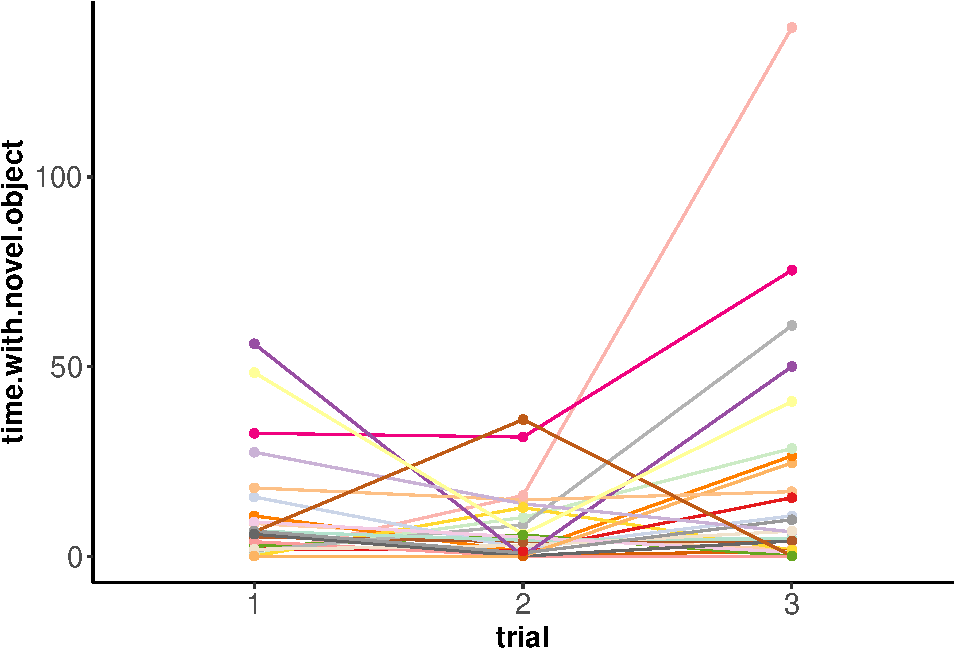
\includegraphics{nov-4-2020-lab-meeting-on-analyses_files/figure-latex/unnamed-chunk-36-1.pdf}

\begin{Shaded}
\begin{Highlighting}[]
\CommentTok{# Repeatability of time spent near both objects at baseline }
\NormalTok{time.near.both.objects.rpt =}\StringTok{ }
\StringTok{  }\KeywordTok{rpt}\NormalTok{(time.with.both.objects }\OperatorTok{~}\StringTok{ }\NormalTok{(}\DecValTok{1} \OperatorTok{|}\StringTok{ }\NormalTok{id), }\DataTypeTok{grname =} \StringTok{"id"}\NormalTok{, }\DataTypeTok{datatype =} \StringTok{"Gaussian"}\NormalTok{,}
      \DataTypeTok{data =}\NormalTok{ baseline.data, }\DataTypeTok{nboot =} \DecValTok{50}\NormalTok{ , }\DataTypeTok{npermut =} \DecValTok{0}\NormalTok{) }
\end{Highlighting}
\end{Shaded}

However, the time spent near \emph{both} objects is significantly
repeatable R = 0.223(95\% CI = 0, 0.477, p = 0.047).

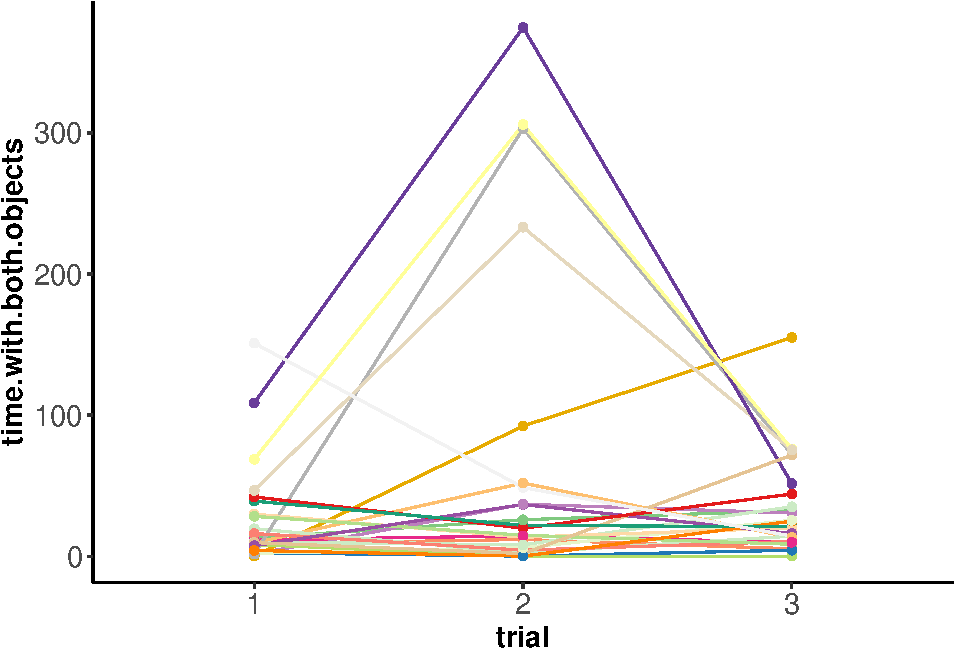
\includegraphics{nov-4-2020-lab-meeting-on-analyses_files/figure-latex/unnamed-chunk-39-1.pdf}

\chapter{Model 2 - Preference for the rewarded object during
training}\label{model-2---preference-for-the-rewarded-object-during-training}

To see whether fish were responsive during training our second model
asks whether the preference for the rewarding object changes throughout
training between the treatments.

\begin{Shaded}
\begin{Highlighting}[]
\NormalTok{training.data.model2 <-}\StringTok{ }
\StringTok{  }\KeywordTok{lmer}\NormalTok{(rewarding.object.preference }\OperatorTok{~}\StringTok{ }\NormalTok{treatment }\OperatorTok{*}\StringTok{ }\NormalTok{trial }\OperatorTok{+}\StringTok{ }\NormalTok{(}\DecValTok{1}\OperatorTok{|}\NormalTok{id), }
       \DataTypeTok{data =}\NormalTok{ training.data)}
\end{Highlighting}
\end{Shaded}

\begin{verbatim}
## # A tibble: 3 x 6
##   term                 estimate std.error statistic    df p.value
##   <chr>                   <dbl>     <dbl>     <dbl> <dbl> <chr>  
## 1 treatmentnovel          8.97      62.4      0.144  34.3 0.886  
## 2 trial                   6.21       1.72     3.60  397.  < .001 
## 3 treatmentnovel:trial    0.417      2.68     0.155 399.  0.877
\end{verbatim}

Throughout training, over the 20 trials, guppies increased their
relative preference for the rewarded object by 6.21 seconds each trial
(Figure \ref{fig:novel-pref-plot}, p \textless{} .001) with no effect of
treatment on performance during training (p = 0.886) suggesting that
whether a guppy was trained to familiar objects or novel objects did not
influence how individuals behaved towards the rewarding object
throughout training.

\begin{figure}
\centering
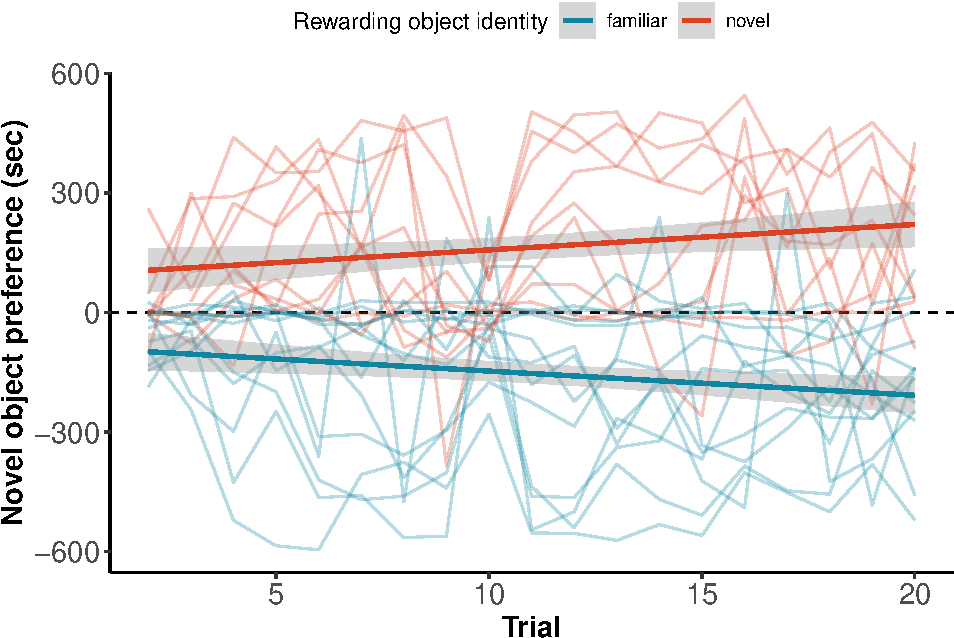
\includegraphics{nov-4-2020-lab-meeting-on-analyses_files/figure-latex/novel-pref-plot2-1.pdf}
\caption{\label{fig:novel-pref-plot2}Preference for the novel object in both
treatments. Negative values represent more time spent with the familiar
object, positive values indicate more time spent with the novel object.
Faded lines connect individuals across trials and solid lines represents
a linear fit with 95\% CI (grey shading).}
\end{figure}

\chapter{Model 3a - Preference for the novel during testing based on
treatment}\label{model-3a---preference-for-the-novel-during-testing-based-on-treatment}

For the main effects of training and treatment on novel object
preference we fit a linear mixed model with fixed effects of trial
(baseline test vs final test) and rewarding object treatment
(novelty-rewarded vs familiar-rewarded).

\begin{Shaded}
\begin{Highlighting}[]
\NormalTok{test.data =}\StringTok{ }\NormalTok{test.data }\OperatorTok\StringTok{ }\KeywordTok{filter}\NormalTok{(treatment }\OperatorTok{!=}\StringTok{ 'control'}\NormalTok{)}
\NormalTok{test.data.model3a =}\StringTok{ }
\StringTok{  }\KeywordTok{lmer}\NormalTok{(novel.object.preference }\OperatorTok{~}\StringTok{  }\NormalTok{trial.type }\OperatorTok{*}\StringTok{ }\NormalTok{treatment }\OperatorTok{+}\StringTok{ }\NormalTok{(}\DecValTok{1} \OperatorTok{|}\StringTok{ }\NormalTok{id) }\OperatorTok{+}\StringTok{ }\NormalTok{(}\DecValTok{1} \OperatorTok{|}\StringTok{ }\NormalTok{trial), }
       \DataTypeTok{data =}\NormalTok{ test.data)}
\end{Highlighting}
\end{Shaded}

\begin{verbatim}
## boundary (singular) fit: see ?isSingular
\end{verbatim}

\begin{verbatim}
## # A tibble: 3 x 6
##   term                             estimate std.error statistic    df p.value
##   <chr>                               <dbl>     <dbl>     <dbl> <dbl> <chr>  
## 1 trial.typere-test                    9.30      16.3     0.570  128. 0.57   
## 2 treatmentnovel                      -2.99      16.7    -0.179  128. 0.858  
## 3 trial.typere-test:treatmentnovel    37.8       25.0     1.51   128. 0.133
\end{verbatim}

When looking at the novel object preference we find no significant
effects of trial type or treatment, and find no interaction effect.
There is a non-significant trend for an interaction effect of trial type
and tretment whereby guppies that were in the novelty-rewarded treatment
had a novel object preference that was 37.8 seconds stronger than the
novel object preference of guppies in the familiar-rewarded treatment (p
= 0.133).

\begin{figure}
\centering
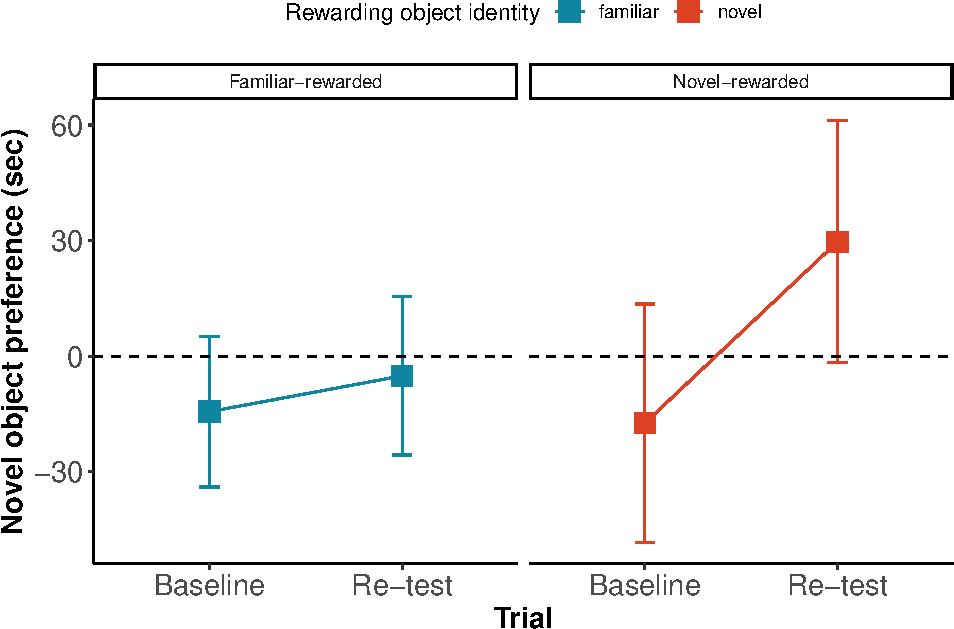
\includegraphics{nov-4-2020-lab-meeting-on-analyses_files/figure-latex/test-data-pref-plot3-1.pdf}
\caption{\label{fig:test-data-pref-plot3}Plot when response is coded as
novel object preference. Data are means +/- 95\% CI.}
\end{figure}

~

\chapter{Model 3b - Preference for the rewarding object during testing
based on
treatment}\label{model-3b---preference-for-the-rewarding-object-during-testing-based-on-treatment}

However, I also ran a model where the response variable is coded as the
rewarding object preference rather than the novel object preference and
this produces different results.

\begin{Shaded}
\begin{Highlighting}[]
\NormalTok{test.data.model3b =}\StringTok{ }
\StringTok{  }\KeywordTok{lmer}\NormalTok{(rewarding.object.preference }\OperatorTok{~}\StringTok{  }\NormalTok{trial.type }\OperatorTok{*}\StringTok{ }\NormalTok{treatment }\OperatorTok{+}\StringTok{ }\NormalTok{(}\DecValTok{1} \OperatorTok{|}\StringTok{ }\NormalTok{id) }\OperatorTok{+}\StringTok{ }\NormalTok{(}\DecValTok{1} \OperatorTok{|}\StringTok{ }\NormalTok{trial), }
       \DataTypeTok{data =}\NormalTok{ test.data)}
\end{Highlighting}
\end{Shaded}

\begin{verbatim}
## boundary (singular) fit: see ?isSingular
\end{verbatim}

\begin{verbatim}
## # A tibble: 3 x 6
##   term                             estimate std.error statistic    df p.value
##   <chr>                               <dbl>     <dbl>     <dbl> <dbl> <chr>  
## 1 trial.typere-test                   -9.30      16.3    -0.570  128. 0.57   
## 2 treatmentnovel                     -31.8       16.7    -1.90   128. 0.059  
## 3 trial.typere-test:treatmentnovel    56.4       25.0     2.25   128. 0.026
\end{verbatim}

When we look at the response variable as the rewarding object preference
(\emph{i.e.} the novel object preference for novelty-trained guppies and
the familiar object preeference for familiar-trained guppies), we find
that there is a significant interaction effect between trial type and
treatment where novelty-trained guppies had a rewarding object
preference that was 56.4 seconds stronger than that of familiar-trained
guppies (p = 0.026).

\begin{figure}
\centering
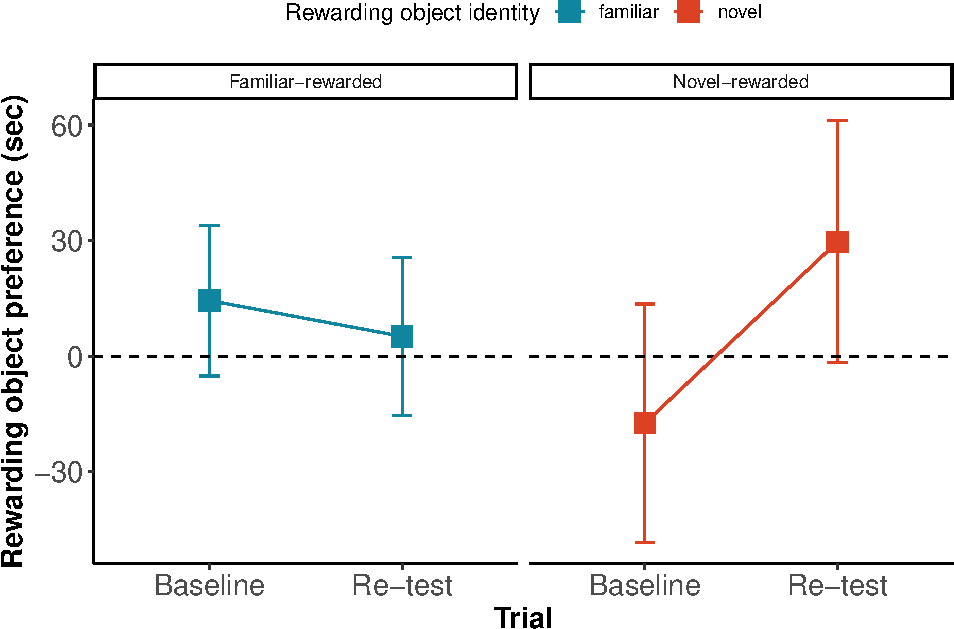
\includegraphics{nov-4-2020-lab-meeting-on-analyses_files/figure-latex/test-data-pref-plot4-1.pdf}
\caption{\label{fig:test-data-pref-plot4}Plot when response is coded as
rewarding object preference. Data are means +/- 95\% CI.}
\end{figure}

It's hard to make out why this is the case. Look at figures 2 and 3
which show the data presented with the different response variables
doesn't make it immediately clear why this should be the case. However,
doing post hoc contrasts for both models (Tables 1 and 2) reveal that
the main contrasts we are interested in are the same between both
models, there is a trend for novelty-trained guppies to increase their
novel object preference (p = 0.07 and same effect size in both models).

\begin{table}

\caption{\label{tab:contrasts-table3}Pairwise contrasts when response variable is coded as rewarding object}
\centering
\begin{tabular}[t]{l|r|r|r|r|l}
\hline
contrast & estimate & df & lower.CL & upper.CL & p.value\\
\hline
baseline familiar - (re-test familiar) & 9.303 & 109.258 & -33.362 & 51.969 & 0.941\\
\hline
baseline familiar - baseline novel & 31.837 & 65.377 & -12.227 & 75.901 & 0.236\\
\hline
baseline familiar - (re-test novel) & -15.266 & 65.377 & -63.855 & 33.324 & 0.841\\
\hline
(re-test familiar) - baseline novel & 22.534 & 65.377 & -22.416 & 67.484 & 0.553\\
\hline
(re-test familiar) - (re-test novel) & -24.569 & 65.377 & -73.963 & 24.826 & 0.559\\
\hline
baseline novel - (re-test novel) & -47.103 & 119.922 & -96.741 & 2.535 & 0.07\\
\hline
\end{tabular}
\end{table}

~

\begin{table}

\caption{\label{tab:contrasts-table4}Pairwise contrasts when response variable is coded as novel object}
\centering
\begin{tabular}[t]{l|r|r|r|r|l}
\hline
contrast & estimate & df & lower.CL & upper.CL & p.value\\
\hline
baseline familiar - (re-test familiar) & -9.303 & 109.258 & -51.969 & 33.362 & 0.941\\
\hline
baseline familiar - baseline novel & 2.987 & 65.377 & -41.077 & 47.051 & 0.998\\
\hline
baseline familiar - (re-test novel) & -44.116 & 65.377 & -92.706 & 4.474 & 0.088\\
\hline
(re-test familiar) - baseline novel & 12.290 & 65.377 & -32.660 & 57.240 & 0.888\\
\hline
(re-test familiar) - (re-test novel) & -34.813 & 65.377 & -84.207 & 14.581 & 0.256\\
\hline
baseline novel - (re-test novel) & -47.103 & 119.922 & -96.741 & 2.535 & 0.07\\
\hline
\end{tabular}
\end{table}

When doing pairwise comparisons, if you do not do all of them it lowers
the p-value since it is less tests. But it is not clear whether I should
do all the pairwise comparisons or just the ones I knew I wanted to do
from the start.

\chapter{Re-test repeatabilities}\label{re-test-repeatabilities}

\begin{Shaded}
\begin{Highlighting}[]
\CommentTok{# Repeatability of activity at re-test }
\NormalTok{activity.repeatability.retest =}\StringTok{ }
\StringTok{  }\KeywordTok{rpt}\NormalTok{(distance.moved }\OperatorTok{~}\StringTok{ }\NormalTok{(}\DecValTok{1} \OperatorTok{|}\StringTok{ }\NormalTok{id), }\DataTypeTok{grname =} \StringTok{"id"}\NormalTok{, }\DataTypeTok{datatype =} \StringTok{"Gaussian"}\NormalTok{, }
      \DataTypeTok{data =}\NormalTok{ retest.data, }\DataTypeTok{nboot =} \DecValTok{50}\NormalTok{ , }\DataTypeTok{npermut =} \DecValTok{0}\NormalTok{) }
\end{Highlighting}
\end{Shaded}

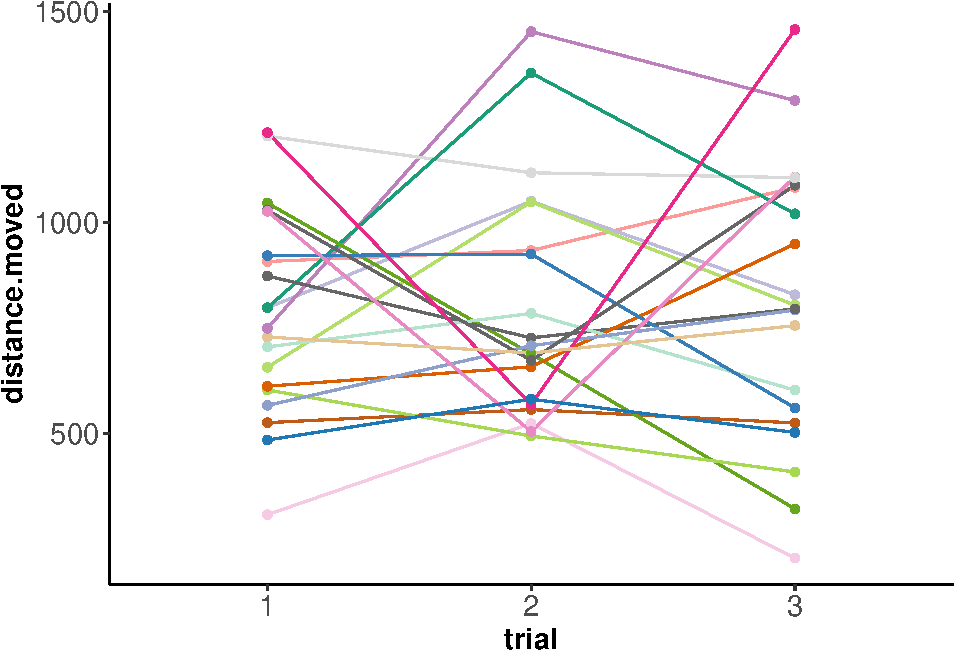
\includegraphics{nov-4-2020-lab-meeting-on-analyses_files/figure-latex/unnamed-chunk-49-1.pdf}

General activity becomes more repeatable at re-test R = 0.425 (95\% CI =
0.208, 0.673, p = 0.001)

\begin{Shaded}
\begin{Highlighting}[]
\CommentTok{# Repeatability of novel object preference at re-test }
\NormalTok{novel.object.pref.rpt.retest =}\StringTok{ }
\StringTok{  }\KeywordTok{rpt}\NormalTok{(time.with.novel.object }\OperatorTok{~}\StringTok{ }\NormalTok{(}\DecValTok{1} \OperatorTok{|}\StringTok{ }\NormalTok{id), }\DataTypeTok{grname =} \StringTok{"id"}\NormalTok{, }\DataTypeTok{datatype =} \StringTok{"Gaussian"}\NormalTok{, }
      \DataTypeTok{data =}\NormalTok{ retest.data, }\DataTypeTok{nboot =} \DecValTok{50}\NormalTok{ , }\DataTypeTok{npermut =} \DecValTok{0}\NormalTok{) }
\end{Highlighting}
\end{Shaded}

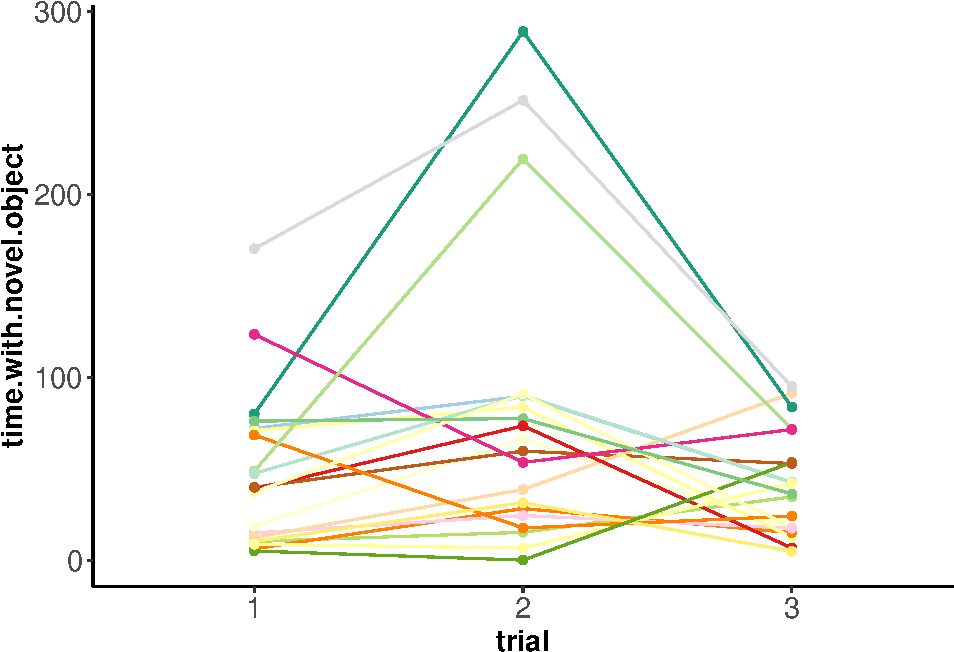
\includegraphics{nov-4-2020-lab-meeting-on-analyses_files/figure-latex/unnamed-chunk-52-1.pdf}

At re-test the time with spent near the novel object is repeatable R =
0.375 (95\% CI = 0.073, 0.623, p = 0.004). It is interesting to note
that time spent near the novel object is not rerpeatable at baseline but
training induces consistency in time spent near a novel object.

\begin{Shaded}
\begin{Highlighting}[]
\CommentTok{# Repeatability of time spent near both objects at re-test }
\NormalTok{time.with.both.objects.rpt.retest =}\StringTok{ }
\StringTok{  }\KeywordTok{rpt}\NormalTok{(time.with.both.objects }\OperatorTok{~}\StringTok{ }\NormalTok{(}\DecValTok{1} \OperatorTok{|}\StringTok{ }\NormalTok{id), }\DataTypeTok{grname =} \StringTok{"id"}\NormalTok{, }\DataTypeTok{datatype =} \StringTok{"Gaussian"}\NormalTok{, }
      \DataTypeTok{data =}\NormalTok{ retest.data, }\DataTypeTok{nboot =} \DecValTok{50}\NormalTok{ , }\DataTypeTok{npermut =} \DecValTok{0}\NormalTok{) }
\end{Highlighting}
\end{Shaded}

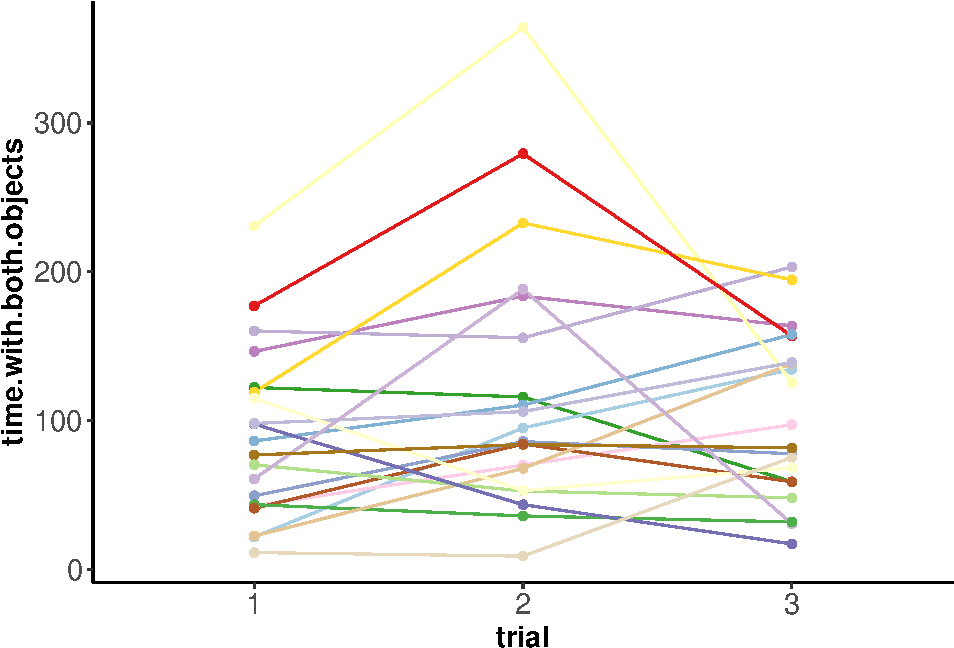
\includegraphics{nov-4-2020-lab-meeting-on-analyses_files/figure-latex/unnamed-chunk-54-1.pdf}

Moreover, the time spent near both objects becomes highly repeatable at
re-test R = 0.536 (95\% CI = 0.088, 0.72, p = 0). \textbf{However, the
novel object preference metric (time spent near novel object subtracted
by time spent near familiar object) is still not repeatable at re-test}.

\chapter{Model 4 - Preference for the rewarding object during training
based on
feeding}\label{model-4---preference-for-the-rewarding-object-during-training-based-on-feeding}

Our fourth model asks whether the time spent near the rewarding object
during a training session is influenced by whether a fish ate or not.

\begin{Shaded}
\begin{Highlighting}[]
\NormalTok{training.data.model.rewarding.object4 =}\StringTok{ }
\StringTok{  }\KeywordTok{lmer}\NormalTok{(rewarding.object.preference }\OperatorTok{~}\StringTok{ }\NormalTok{ate }\OperatorTok{+}\StringTok{ }\NormalTok{(}\DecValTok{1} \OperatorTok{|}\StringTok{ }\NormalTok{id) }\OperatorTok{+}\StringTok{ }\NormalTok{(}\DecValTok{1}\OperatorTok{|}\StringTok{ }\NormalTok{trial), }
       \DataTypeTok{data =}\NormalTok{ training.data)}
\end{Highlighting}
\end{Shaded}

\begin{verbatim}
## # A tibble: 1 x 6
##   term  estimate std.error statistic    df p.value
##   <chr>    <dbl>     <dbl>     <dbl> <dbl> <chr>  
## 1 ateY      165.      18.9      8.72  363. < .001
\end{verbatim}

Throughout all of training, fish that ate during a session spent on
average 164.9 more seconds near the rewarded object compared to fish
that did not eat (Figure, \ref{fig:training-data-ate-plot}, p
\textless{} .001).

\begin{figure}
\centering
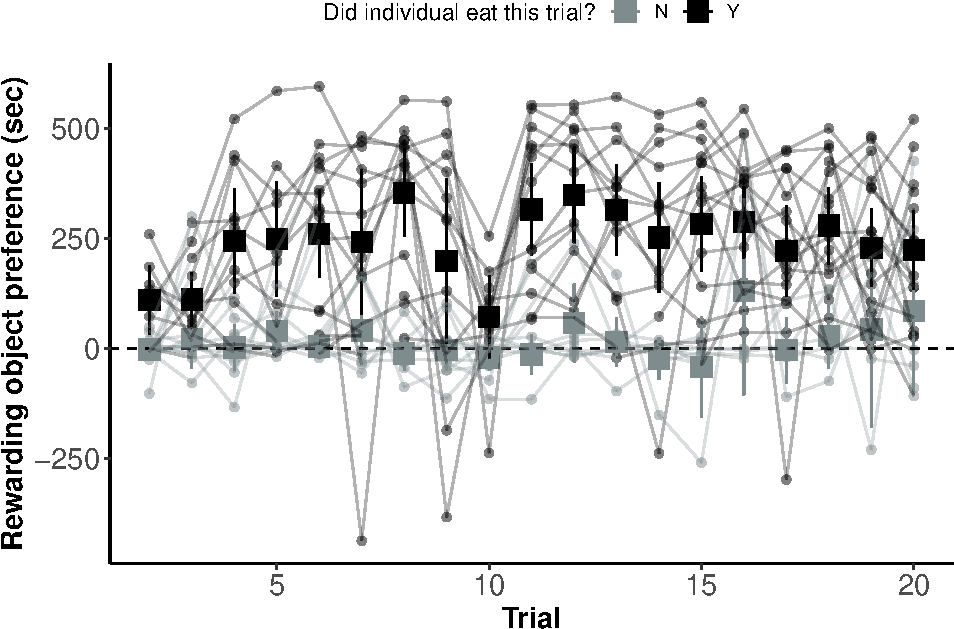
\includegraphics{nov-4-2020-lab-meeting-on-analyses_files/figure-latex/training-data-ate-plot2-1.pdf}
\caption{\label{fig:training-data-ate-plot2}Preference for the rewarding
object during training based on whether an individual ate during a trial
or not. Dashed line represents the no preference value. Data are means
+/- 95\% CI.}
\end{figure}

This is consistent with the results of project 2 where I tried to shift
coloured object preferences. In that experiment trials lasted 5 minutes
and fish that ate spent 91.2 seconds more near the rewarded object than
fish that did not eat. Trials in this experiment lasted 10 minutes and
we see here that with a 2x trial length fish spent 1x the amount of time
near the rewarded object.

\chapter{Model 5 - Do treatments differ in feeding
activity?}\label{model-5---do-treatments-differ-in-feeding-activity}

A discrepancy in reinforcement between treatments may influence
performance on a final preference test. To see whether there was a
difference in feeding between treatments I counted the number of trials
in which an individual fish ate throughout all of training and compared
the feeding counts between treatments. To do this I fit a generalized
linear model with a Poisson distribution.

\begin{Shaded}
\begin{Highlighting}[]
\NormalTok{feeding.data.model5 =}\StringTok{ }
\StringTok{  }\KeywordTok{glm}\NormalTok{(feeding.count }\OperatorTok{~}\StringTok{ }\NormalTok{treatment, }\DataTypeTok{family =} \StringTok{"poisson"}\NormalTok{, }
      \DataTypeTok{data =}\NormalTok{ my.feeding.data)}
\end{Highlighting}
\end{Shaded}

The response variable `feeding count' is a sum of the number of trials
in which a guppy ate and the fixed effect `object' represents the
rewarding object identity.

\begin{verbatim}
## # A tibble: 1 x 5
##   term           estimate std.error statistic p.value
##   <chr>             <dbl>     <dbl>     <dbl> <chr>  
## 1 treatmentnovel  -0.0617     0.135    -0.457 0.648
\end{verbatim}

I find no significant difference in the amount of feeding done by
individuals trained to green versus individuals trained to blue (Figure
\ref{fig:feeding-count-plot2}, p = 0.648) which suggests that the
observed group-level differences in final test performance between
blue-trained guppies versus green-trained guppies cannot be explained by
differences in performance during training.

\begin{figure}
\centering
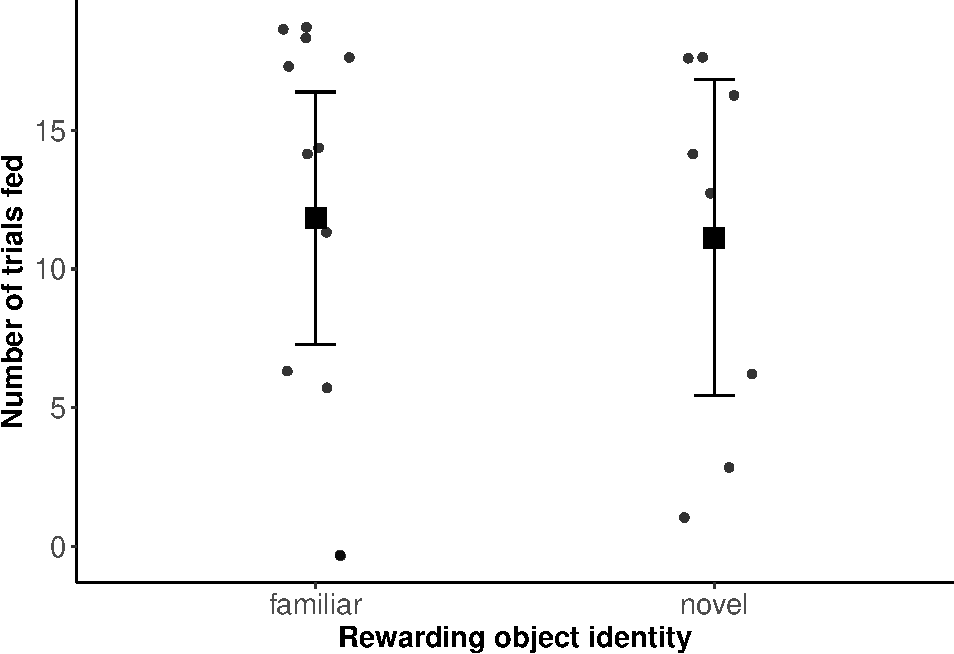
\includegraphics{nov-4-2020-lab-meeting-on-analyses_files/figure-latex/feeding-count-plot2-1.pdf}
\caption{\label{fig:feeding-count-plot2}Average number of trials in which a
fish fed during training}
\end{figure}

\chapter{Controlling for feeding
count}\label{controlling-for-feeding-count}

\emph{Rewarding object preference}

\begin{Shaded}
\begin{Highlighting}[]
\NormalTok{test.data.feeding.controlled.model6 =}\StringTok{ }
\StringTok{  }\KeywordTok{lmer}\NormalTok{(rewarding.object.preference }\OperatorTok{~}\StringTok{ }\NormalTok{trial.type }\OperatorTok{*}\StringTok{ }\NormalTok{treatment }\OperatorTok{+}\StringTok{ }\NormalTok{feeding.count }\OperatorTok{+}\StringTok{ }\NormalTok{(}\DecValTok{1}\OperatorTok{|}\NormalTok{id) }\OperatorTok{+}\StringTok{ }\NormalTok{(}\DecValTok{1}\OperatorTok{|}\NormalTok{trial), }
       \DataTypeTok{data =}\NormalTok{ test.feeding.data)}
\end{Highlighting}
\end{Shaded}

\begin{verbatim}
## boundary (singular) fit: see ?isSingular
\end{verbatim}

\begin{verbatim}
## # A tibble: 4 x 6
##   term                             estimate std.error statistic    df p.value
##   <chr>                               <dbl>     <dbl>     <dbl> <dbl> <chr>  
## 1 trial.typere-test                   -8.78    16.3      -0.540  127. 0.59   
## 2 treatmentnovel                     -27.2     16.9      -1.61   127. 0.111  
## 3 feeding.count                        1.31     0.912     1.44   127. 0.152  
## 4 trial.typere-test:treatmentnovel    52.7     25.0       2.11   127. 0.037
\end{verbatim}

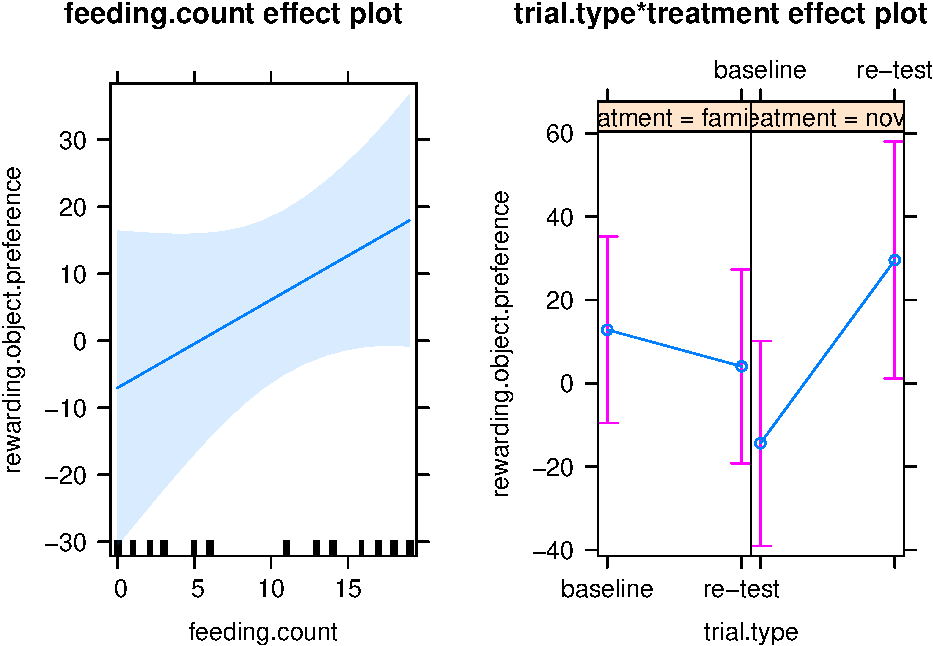
\includegraphics{nov-4-2020-lab-meeting-on-analyses_files/figure-latex/unnamed-chunk-63-1.pdf}

Testing for an effect of feeding count on rewarding object preference
finds that there is no significant effect but the effect is in the
expected direction and including feeding count as a covariate in model
3b does not change the results.

There is an effect of feeding on the time spent near \textbf{both}
objects. Looking at the effect predictions of the model a fish that
would have 0 feedings would spend -7.039 seconds near both objects
whereas a fish that fed in 19 trials would spend 17.914 seconds near
both objects, a -2.5-fold increase. This result is highly consistent
with the one seen in the previous colour learning experiment. A
significant effect of number of trials fed on time spent near both
objects and a non-significant trend for feeding count to increase the
preference for the rewarding object.

Given that the time spent near both objects is highly repeatable and
that the time spent near both objects is influenced by feeding during
training and that there is no effect of treatment (but there is a trend,
see models 3a and 3b) it seems that the guppies are becoming responsive
to training but not discriminating the objects they spend time with,
choosing instead to spend more time with all objects regardless of
identity.

\chapter{Why so little power}\label{why-so-little-power}

\begin{figure}
\centering
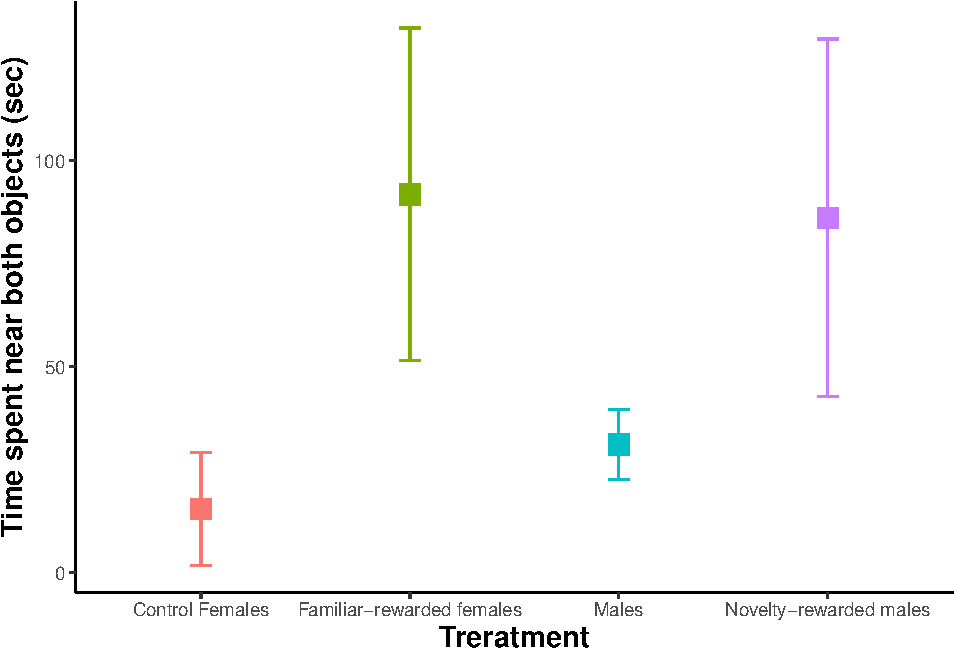
\includegraphics{nov-4-2020-lab-meeting-on-analyses_files/figure-latex/control-plot3-1.pdf}
\caption{\label{fig:control-plot3}Time near both objects at re-test for
females and males of various treatments}
\end{figure}

\bibliography{book.bib,packages.bib}

\end{document}
